\documentclass[12pt, spanish, pdftex]{UC3M_document}

%%%%% Preamble %%%%%
\author{Jorge Rodríguez Fraile}
\authorstwotrue
\authorsuptothree{Jorge Rodríguez Fraile}{100405951}{Grupo 83}{}{}{}{}{}{}


%%%%% Basic data about the document (Degree, subject, title, campus, page number custom text) %%%%%
\documentdata{Grado en Ingeniería Informática}{Algoritmos Genéticos y Evolutivos}{Práctica 1 \\ Optimización de Sensores en Smart Cities}{Leganés}{}

%%%%% Page style %%%%%
\header
\footer
\pagestyle{fancy}

\begin{document}
%%%%% Page title %%%%%
\begin{titlepage}
	\centeredtitle{img/LogoUC3M.png}{\studyname}{Curso 2021-2022}{\subjectname}{\documenttitle}
	
	\begin{table}[b]
		\centering
		\begin{tabular}{ cccc }
			\large Jorge Rodríguez Fraile & \large 100405951 & \large Grupo 83 & \href{mailto:100405951@alumnos.uc3m.es}{\large 100405951@alumnos.uc3m.es} \\
			                              &                  &                 &                                                                           \\
			                              &                  &                 &                                                                           \\
		\end{tabular}
	\end{table}
	
\end{titlepage}

\newpage

%%%%% Index %%%%%
\begin{spacing}{0.5}
	% \shipout\null                   % Blank page before index (after title page)
	\hypersetup{linkcolor=black}    % References/links on the index will remain black color
	\tableofcontents\newpage        % Index of the document
	\listoffigures\newpage          % Index of pictures
	\listoftables\newpage           % Index of tables
\end{spacing}


%%%%% DOCUMENT CONTENT %%%%%
\section{Introducción}
En los últimos años ha aumentado mucho el interés por las Ciudades Inteligentes o Smart Cities, desde que la mayoría de la población se encuentran en ciudades. La aplicación de la tecnología en las ciudades haciéndolas smart permite mejorar la calidad de vida y reducir el impacto medioambiental.

En este trabajo vamos a tratar de resolver un problema de estaciones de medición de la calidad del aire, que se encuentra en la ciudad de Madrid que posee 24 estaciones que miden 16 variables ambientales distintas. El problema consiste en el mantenimiento e instalación de las estaciones de medición, que suponen un gran gasto, de lo que se tratara es de determinar que sensores de los presentes en las estaciones deben estar activos para poder reducir el coste y no perder precisión en las mediciones.

\section{Codificación y Función de fitness}
Al tratarse de 24 estaciones en las que puede haber hasta 16 tipos de sensores, la representación que se ha elegido es binaria. Cada uno de los cromosomas estará representado por $24 \cdot 16=384$ bits o genes de manera que cada 16 bits sea una estación distinta, se empezará por el primer sensor de la primera estación, después el segundo sensor y así hasta el último de la primera para dar paso a la siguiente estación. El valor 1 de un bit indicará que se instala el sensor y 0 que no se instala, en cuanto al sensor que representa cada bit son los siguientes:
\begin{table}[H]
	\centering
	\caption{Medidas de los sensores}
	\begin{tabular}{|l|l|l|l|}
		\hline
		1  & Dióxido de Azufre           & SO$_2$ & µg/m$^3$ \\ \hline
		2  & Monóxido de Carbono         & CO     & µg/m$^3$ \\ \hline
		3  & Monóxido de Nitrógeno       & NO     & µg/m$^3$ \\ \hline
		4  & Dióxido de Nitrógeno        & NO$_2$ & µg/m$^3$ \\ \hline
		5  & Partículas \textless 2.5 µm & PM2.5  & µg/m$^3$ \\ \hline
		6  & Partículas \textless 10 µm  & PM10   & µg/m$^3$ \\ \hline
		7  & Óxidos de Nitrógeno         & NOx    & µg/m$^3$ \\ \hline
		8  & Ozono                       & O$_3$  & µg/m$^3$ \\ \hline
		9  & Tolueno                     & TOL    & µg/m$^3$ \\ \hline
		10 & Benceno                     & BEN    & µg/m$^3$ \\ \hline
		11 & Etilbenceno                 & EBE    & µg/m$^3$ \\ \hline
		12 & Metaxileno                  & MXY    & µg/m$^3$ \\ \hline
		13 & Paraxileno                  & PXY    & µg/m$^3$ \\ \hline
		14 & Ortoxileno                  & OXY    & µg/m$^3$ \\ \hline
		15 & Hexano (total)              & TCH    & mg/m$^3$ \\ \hline
		16 & Hexano (no metánicos)       & NMHC   & mg/m$^3$ \\ \hline
	\end{tabular}
\end{table}
Ejemplo: 0010010100000000 0000000000000000 … \\ Indica que en la primera estación se instalan los sensores de NO, PM10 y O$_3$, sin embargo en la estación 3 ni siguiera se instala al no tener sensores.
\pagebreak

En cuanto a la función de evaluación que se empleará será $f=\frac {precio} {calidad}$ que será calculada mediante un servidor al que podremos proporcionarle un cromosoma y recibir el resultado. La función representa el precio por unidad de calidad, nosotros al buscar recibir la mayor calidad de la manera más barata trataremos de minimizar este valor.

En las secciones posteriores se tratará de resolver el problema mediante dos enfoques diferentes, uno más tradicional mediante fuerza bruta y otro mediante algoritmos genéticos.

\section{Programación enfoque clásico}
Esta primera aproximación se realizará sobre el problema reducido, en vez de tratar con 24 estaciones se realizará solo con 1 dado que como se resolverá mediante fuerza bruta cada bit de más multiplica el número de posibilidades y tiempo de ejecución por 2, este aumento haría incalculable en un tiempo razonable las 24 estaciones.

El programa ha realizado sobre Python y consiste en lo siguiente:
\begin{itemize}
	\item Partir del cromosoma semilla, 0000000000000000.
	\item Evaluar el cromosoma mediante una petición de get al servidor para obtener el valor de la función de fitness. Se va guardando el número de evaluación, cromosoma y valor de fitness más pequeño obtenido, que se escribe en un fichero de registro.
	\item Aumentar el cromosoma, en este caso le sumamos 1 en binario, ya que evaluaremos todas las posibilidades del cromosoma.
	\item Cuando se haya llegado al 1111111111111111 se parará el proceso y se sacara por pantalla en número de evaluaciones (aunque se sabe de antemano), la evaluación de mejor fitness, el mejor cromosoma y su valor de fitness.
\end{itemize}

La salida que obtenemos para la primera estación es el cromosoma \textbf{0000100111110110} que se obtiene en la evaluación número \textbf{2551} con un fitness de \textbf{10403,58}. Para obtener este resultado se han realizado un total de \textbf{65536} evaluaciones. A continuación se puede ver el progreso de la función de fitness a lo largo de los ciclos (aumentando en 1 el valor del cromosoma) con respecto al mejor resultado (menor valor de fitness) obtenido hasta el ciclo:
\begin{figure}[H]
	\ffigbox[\FBwidth]
	{\caption{Función de fitness vs. Evaluaciones}}
	{\def\svgwidth{.95\textwidth}
		\input{./img/brute-force.pdf_tex}}
\end{figure}
\vspace{-.7cm}
Como se puede ver al realizarlo por fuerza bruta sin ningún tipo de heurística o sentido de si va en buena dirección. Los valores de fitness según progresan las evaluaciones van subiendo y bajando, suben según se van activando más sensores y al saltar a un 1 bit más da una bajada, al volver los valores a 0. Como la mejor evaluación es temprana se puede ver que se mantiene a lo largo de casi todo el proceso, aun obteniéndose pronto seguimos porque puede haber otra mejor, aunque finalmente no lo haya.

\section{Programación Algoritmos Genéticos}
Esta segunda parte…

\subsection{Operadores genéticos}

Selección

Cruce

Mutación

Remplazo

\subsection{Pruebas}
Para empezar, los modelos  se han nombrado siguiendo una codificación con el siguiente formato XX\_YY\_ZZ, tal que:
\begin{itemize}
	\item XX: Número de generaciones generadas.
	\item YY: Tamaño del conjunto de candidatos al hacer torneo para la selección.
	\item ZZ: Porcentaje de mutaciones sobre la población.
\end{itemize}

Una vez aclarado esto podemos dar paso a los primeros modelos de prueba. Los parámetros seleccionados para estas primeras pruebas han sido 100 generaciones para cada uno, tamaños de torneo de 10, 20 y 34 individuos y porcentaje de mutación de 1 \% y 5 \%. Para dar consistencia a los resultados y evitar que por probabilidad hayan podido salir mejores o peores resultados se han realizado 5 ejecuciones para cada uno de estos modelos y se ha hecho la media. En el siguiente gráfico se pueden ver estos 6 modelos:

\begin{figure}[H]
	\ffigbox[\FBwidth]
	{\caption{Fitness primeros modelos}}
	{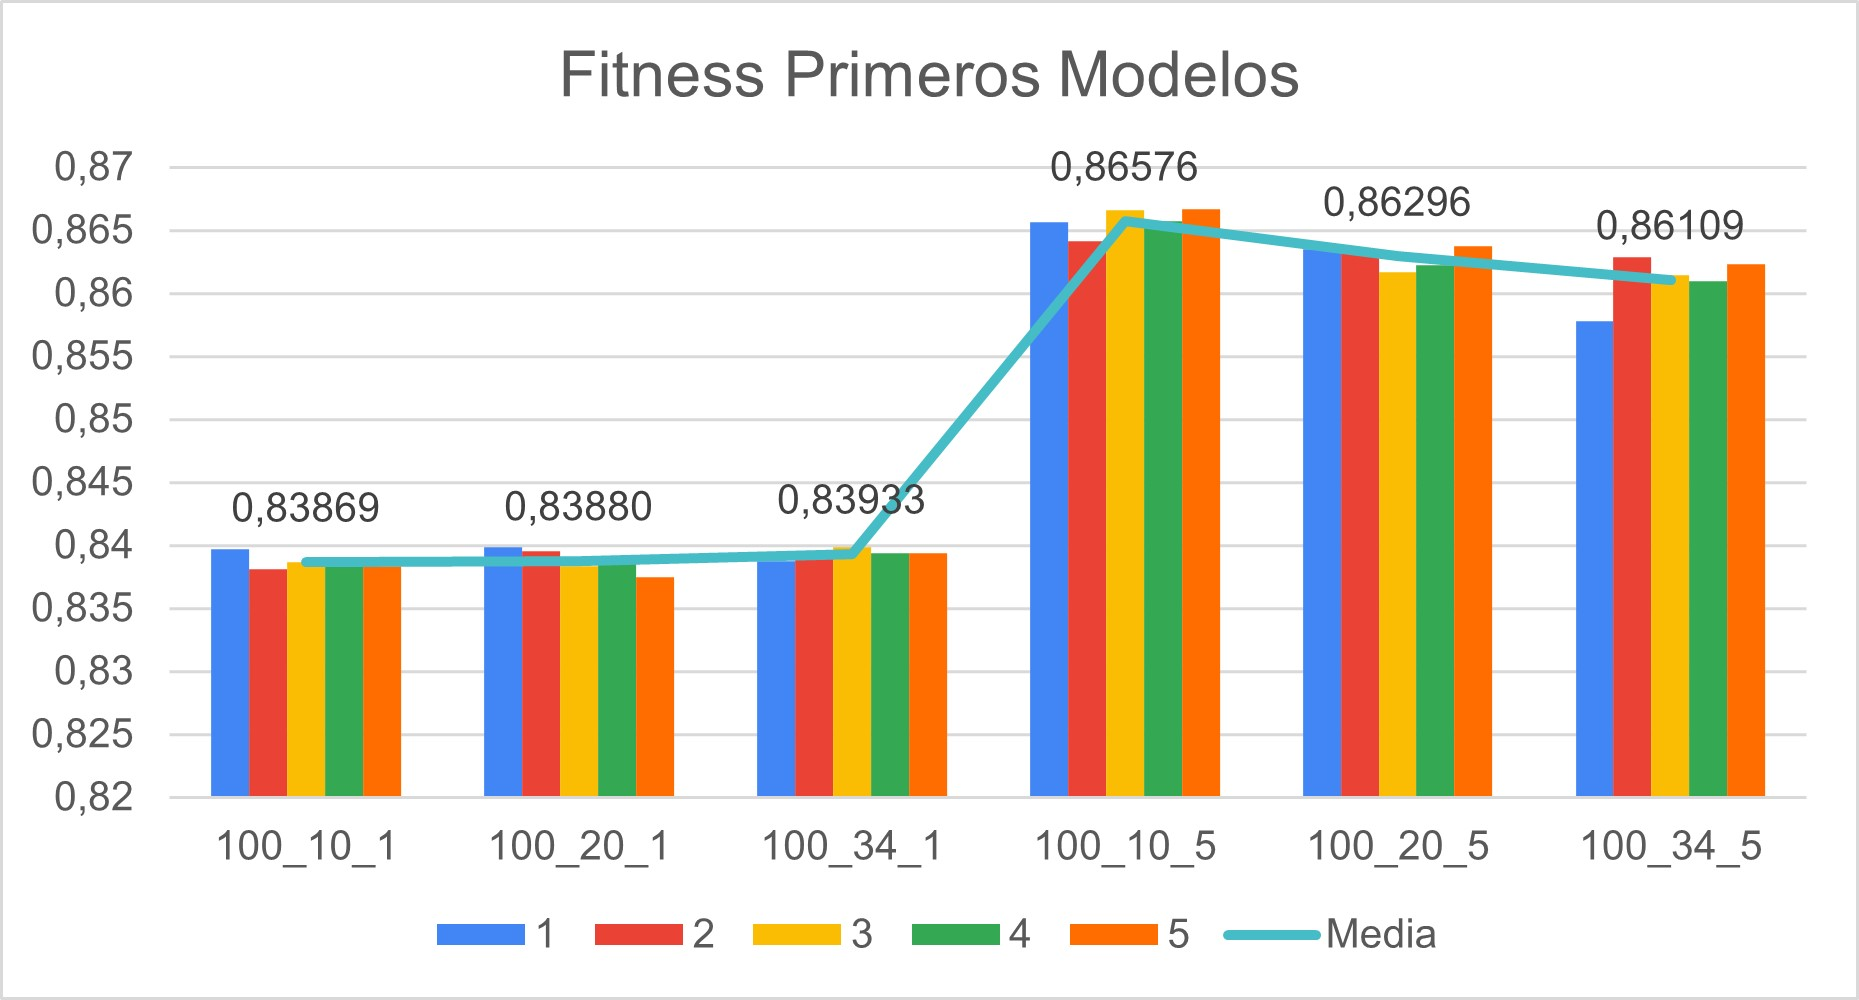
\includegraphics[scale=.8]{./img/first_models.jpg}}
\end{figure}

Podemos ver que en general aumentar el porcentaje de mutaciones empeora los resultados y que dentro de aquellos con un 1 \% de mutaciones el mejor aunque no por mucho es el de menor tamaño de torneo, 10 individuos, hasta este punto el mejor resultado ha sido el modelo 100\_10\_1 con un fitness de 0,838089054 en 10100 evaluaciones. Se puede ver a continuación que el fitness ha ido bajando más rápido al principio y que se ha estabilizado al final por lo que las 100 generaciones son todavía suficientes. 

\begin{figure}[H]
	\ffigbox[\FBwidth]
	{\caption{Fitness vs Evaluaciones 100\_10\_1}}
	{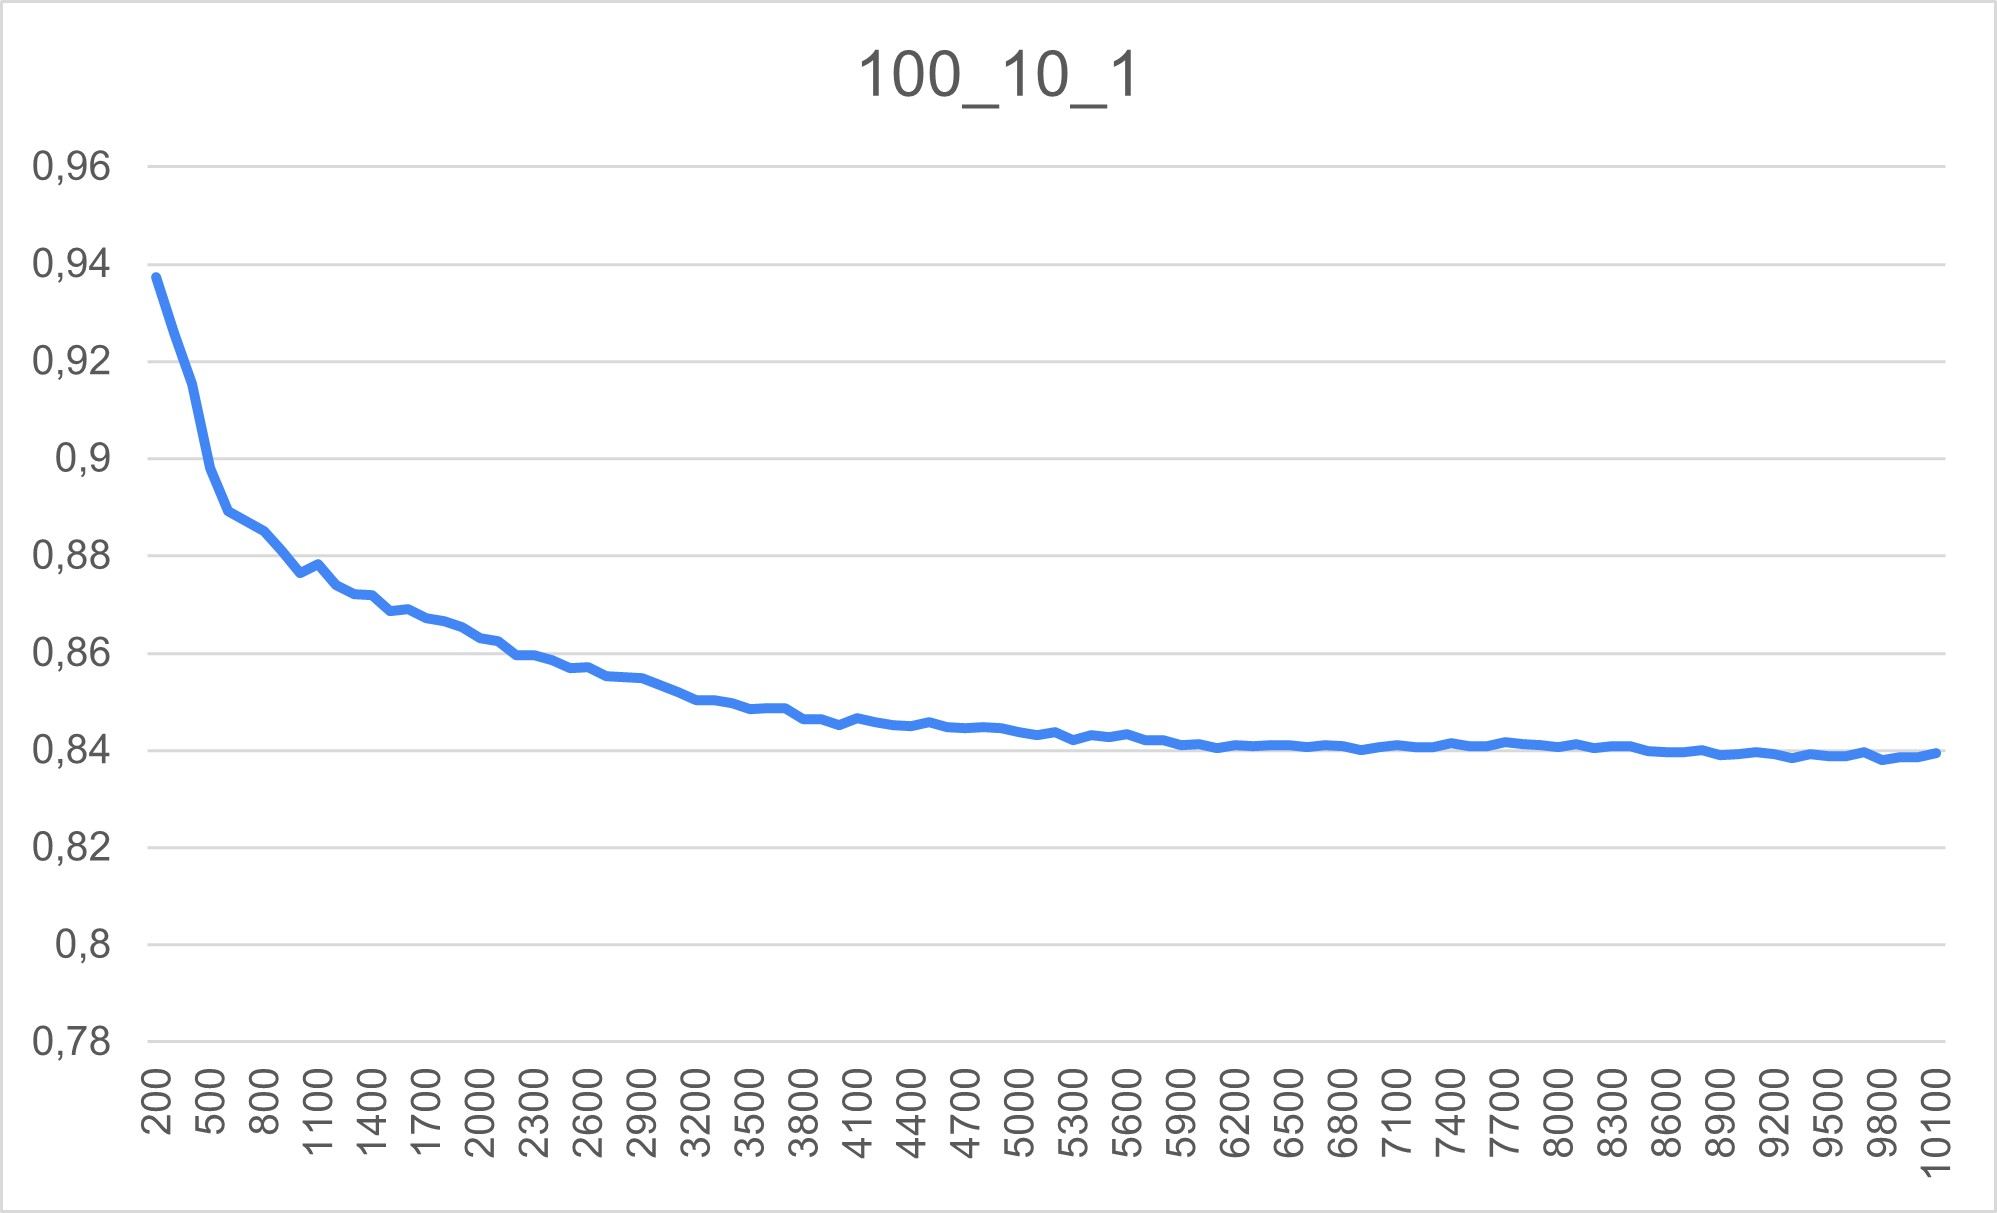
\includegraphics[scale=.65]{./img/100_10_1.jpg}}
\end{figure}

En vista de los resultados anteriores, se va a probar primero a reducir los tamaños de torneo a 6 y 4 individuos, se ha aumentado el número de generaciones (150) para que puedan seguir convergiendo con normalidad. En la siguiente grafica se pueden ver los resultados nuevos comparados con los previos para un tamaño diferente de torneo:

GRAFICA


Podemos apreciar que ... el mejor es... su grafica


Ahora pasamos a buscar uno de los parámetros más importantes, el valor para la mutación, basado en la mejor prueba anterior se procede a reducir su valor a 0,5, 0,1 y 0,05. Para estas pruebas se ha aumentado el número de generaciones ya que en cada generación se realizan movimientos en el espacio de soluciones más pequeños. A continuación se presentan estos nuevos modelos:

GRAFICA

RESULTADOS TOTALES... PONER EL CROMOSOMA Y SU SIGNIFICADO... PROBAR HASTA 10 VECES
JUSTIFICAR DESPUES DE CADA RESULTADO EL POR QUE



\end{document}